\section{\texttt{Symbol} 型と\texttt{Expr} 型 -- Julia の抽象構文木}
\begin{frame}
  \frametitle{Outline}
  \tableofcontents[currentsection]
\end{frame}

\begin{frame}[containsverbatim]
\frametitle{Julia の抽象構文木(AST)}
\begin{columns}
\begin{column}{.65\linewidth}
  \begin{itemize}
    \item 例えば\verb|x + (y + z)| という式はJulia の中の人からは右図のように木構造(抽象構文木)として見えている
      \begin{itemize}
        \item \verb|:call| は関数呼び出しの意味
        \item \verb|+| は中置が認められているというだけで普通の関数であることに注意
        \item つまり正確には \verb| +(x, +(y, z))|
      \end{itemize}
  \item Julia は式をこのように抽象構文木に変換して、それから式の評価をしている
    \begin{itemize}
      \item この構造をそのまま保持することで、式やプログラムそのものをデータとして扱える(=\textblue{同図像性})
      \item プログラムを生成するプログラムも書ける(=\textblue{メタプログラミング})
    \end{itemize}
  \end{itemize}
\end{column}
\begin{column}{.55\linewidth}
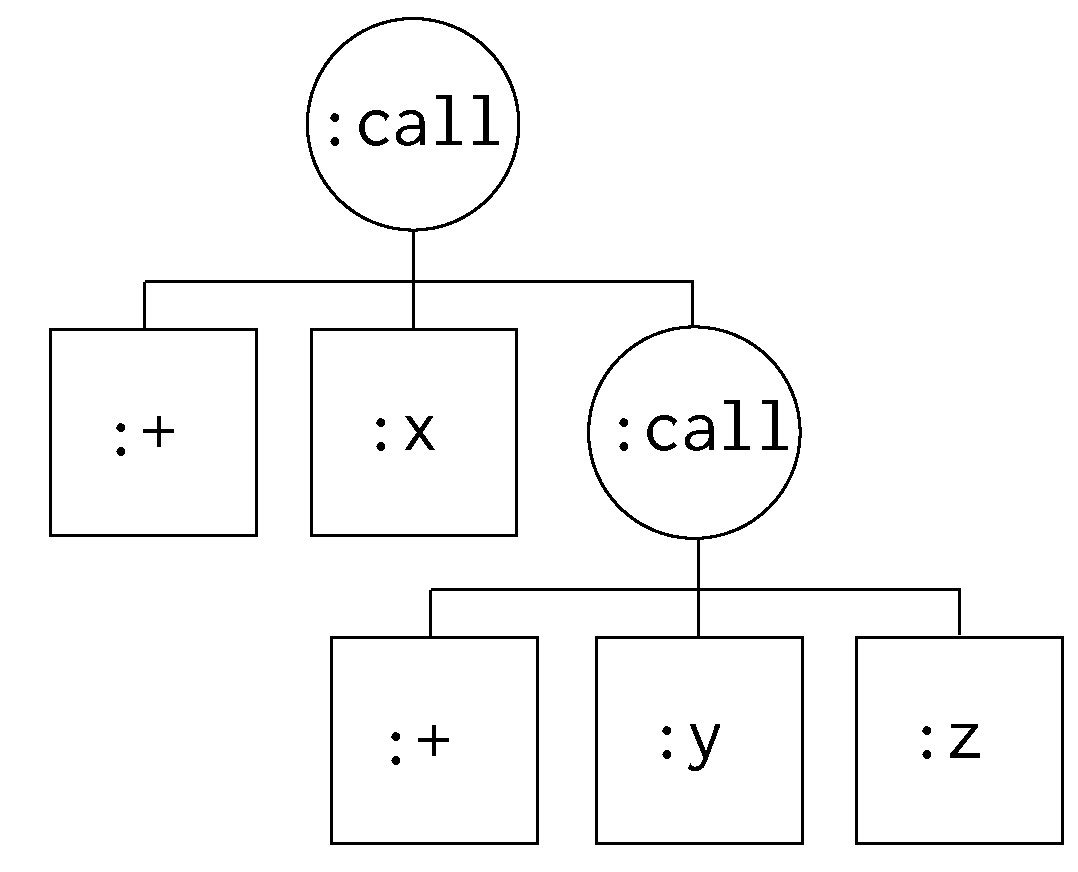
\includegraphics[width=.8\linewidth]{ast.pdf}
\end{column}
\end{columns}
\end{frame}

\begin{frame}[containsverbatim]
\frametitle{Julia の抽象構文木(AST) と\texttt{Symbol}型、 \texttt{Expr}型}
\begin{itemize}
  \item Julia における最も重要な型(データ構造)のうち2つが\verb|Symbol| と\verb|Expr| である
    \begin{itemize}
      \item \verb|Symbol| は識別子・変数名を表す型
      \item \verb|Expr| はJulia そのものの抽象構文木(AST)を表す型
    \end{itemize}
  \item これらの型のオブジェクト(シンボル、AST)は\verb|:()|や\verb|quote ... end| を用いることで作ることができる
\end{itemize}
\begin{lstlisting}
julia> s = :x
:x

julia> typeof(s)
Symbol

julia> ex = :(x + 1)
:(x + 1)

julia> typeof(ex)
Expr
\end{lstlisting}
\end{frame}

\begin{frame}[containsverbatim]
\frametitle{Julia の抽象構文木(AST) と\texttt{Symbol}型、 \texttt{Expr}型}
\begin{itemize}
  \item \verb|Expr| は\verb|head, args, typ| の3つのfield を持つ
    \begin{enumerate}
      \item \verb|head| は行う操作
      \item \verb|args| は操作の対象(引数)
      \item \verb|typ| は結果の型(確定していれば)
        \begin{itemize}
          \item ほとんどの場合で\verb|Any| であり、気にする必要はほとんど無い
        \end{itemize}
    \end{enumerate}
  \item \verb|Base.dump| でまとめて表示できる
    \item \verb|Base.Meta.show_sexpr| を使うとS式で表示できる
\end{itemize}
\begin{lstlisting}
julia> dump(ex)
Expr
  head: Symbol call
  args: Array(Any,(3,))
    1: Symbol +
    2: Symbol x
    3: Int64 1
  typ: Any

julia> Base.Meta.show_sexpr(ex)
(:call, :+, :x, 1)
\end{lstlisting}
\end{frame}

\begin{frame}[containsverbatim]
\frametitle{Julia の抽象構文木(AST) と\texttt{Symbol}型、 \texttt{Expr}型}
\begin{itemize}
  \item AST は木構造なので節と葉を持つ
    \begin{itemize}
      \item 節は\verb|Expr| 型
      \item 葉は\verb|Symbol| 型の値(変数名)かリテラル(数値型・文字列型)
      \item 今回、簡単のため\verb|Expr|, \verb|Symbol|, リテラルをすべてまとめてAST と呼ぶ
    \end{itemize}
\end{itemize}
\begin{lstlisting}
julia> dump( :( x + ( y + z ) ) )
Expr
  head: Symbol call
  args: Array(Any,(3,))
    1: Symbol +
    2: Symbol x
    3: Expr
      head: Symbol call
      args: Array(Any,(3,))
        1: Symbol +
        2: Symbol y
        3: Symbol z
      typ: Any
  typ: Any
\end{lstlisting}
\end{frame}

\begin{frame}[containsverbatim]
\frametitle{変数補間(interpolation)}
\begin{itemize}
  \item quote でAST を作るときに、\verb|$| を使うことで変数や式の値を入れることができる
    \begin{itemize}
      \item 文字列(\verb|" "|)やプロセス(\verb|` `|)における補間と同じ
    \end{itemize}
\end{itemize}
\begin{lstlisting}
julia> y = 42
42

julia> :(x = y)
:(x = y)

julia> :(x = $y)
:(x = 42)

julia> :(x = sin(1.0))
:(x = sin(1.0))

julia> :(x = $(sin(1.0)))
:(x = 0.8414709848078965)
\end{lstlisting}
\end{frame}

\begin{frame}[containsverbatim]
\frametitle{変数補間で\texttt{Symbol} を陽に残す}
\begin{itemize}
  \item 例えば\verb|Symbol| を受け取る関数を呼び出す式をquote したいときに、その\verb|Symbol| を変数補間で与えたい
  \item この時そのまま\verb|$s| と書くと、\verb|Symbol| ではなく名前が書き込まれてしまう
    \begin{itemize}
      \item ほとんどのマクロではこの挙動の方が都合がいい
    \end{itemize}
  \item 配列かタプルに隠して埋め込み、後から取り出せばよい
\end{itemize}

\begin{lstlisting}
julia> :( foo(:a) ) # これが欲しい
:(foo(:a))

julia> s = :a ;
julia> :( foo($s) ) # 直接埋め込むとダメ
:(foo(a))

julia> :( foo( $[s]...) ) # 一度配列に隠す
:(foo([:a]...))

julia> :( foo( $(s,)...) ) # タプルでも良い
:(foo((:a,)...))
\end{lstlisting}

\end{frame}

\begin{frame}[containsverbatim]
\frametitle{式の評価}
\begin{itemize}
  \item \verb|eval| 関数にAST を渡すことで、AST の評価を行える
  \item AST に未定義な変数を含めることができるが、定義する前にAST を評価するともちろんエラーが出る
\end{itemize}
\begin{lstlisting}
julia> x
ERROR: UndefVarError: x not defined

julia> ex = :(2 * x)
:(2x)

julia> eval(ex)
ERROR: UndefVarError: x not defined

julia> x = 42
42

julia> eval(ex)
84
\end{lstlisting}
\end{frame}

\begin{frame}[containsverbatim]
\frametitle{式の操作}
\begin{itemize}
  \item \verb|Expr| は\verb|immutable| ではないので、AST を操作することができる
\end{itemize}
\begin{lstlisting}
julia> ex
:(2x)

julia> x, eval(ex)
(42,84)

julia> ex.args[2] = 20;

julia> ex
:(20x)

julia> x, eval(ex)
(42,840)
\end{lstlisting}
\end{frame}

\begin{frame}[containsverbatim]
\frametitle{第一級オブジェクトとしてのAST \\ -- 同図像性(Homoiconic)}
\begin{itemize}
  \item ソースコードをquote することでAST を生み出すことができた
    \begin{itemize}
      \item \verb|Expr| のコンストラクタを呼び出して作ることもできる
      \item \verb|parse| 関数を使うことで、文字列から作ることもできる
    \end{itemize}
\end{itemize}
\begin{lstlisting}
julia> parse("x+1")
:(x + 1)
\end{lstlisting}
\begin{itemize}
  \item もちろん関数に渡したり関数から受け取ったりできる
  \begin{itemize}
    \item 既に\verb|eval| や\verb|dump|、\verb|parse| といった実例を見てきた
    \item AST を渡すと別のAST に変換する関数を作ることもできる
  \end{itemize}
  \item \verb|eval| に渡すことでいつでもAST を評価・実行できる
  \item このように、自分自身のAST そのものをデータとして扱える言語の性質をhomoiconic と呼ぶ
    \begin{itemize}
      \item AST(プログラム)を自動生成するプログラムを簡単に書ける -- メタプログラミング
      \item マクロを使うことで、より自然な構文の書き換えを行うことができる
    \end{itemize}
\end{itemize}
\end{frame}

